\begin{frame}[t]
  \slideheader{01. INTRODUCTION \& CONTEXT}{The Environment and Reality of Audio Sampling}

  \begin{columns}[onlytextwidth, c]
    % Left Column: Prominent Studio Photograph
    \begin{column}{0.48\textwidth}
      \begin{tcolorbox}[standardcard, top=3pt, bottom=3pt]
        \centering
        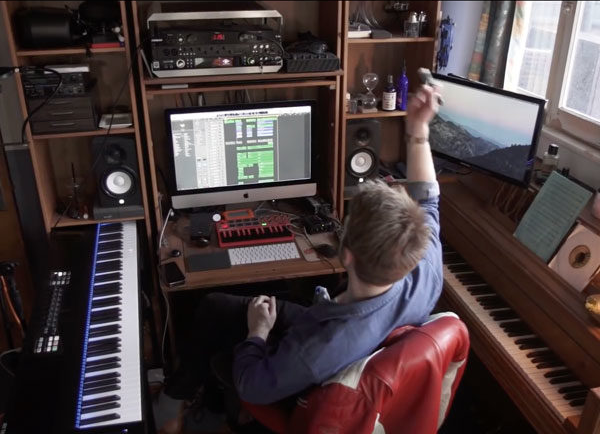
\includegraphics[width=\linewidth, height=4.2cm, keepaspectratio]{images/musician_cropped.png}\par\vspace{1mm}
        {\tiny\textcolor{textdim}{\textbf{Production Context:} Bedroom workstation with DAW, keyboard, and monitoring.}}
      \end{tcolorbox}
    \end{column}

    % Right Column: Definition & Two Key Metrics
    \begin{column}{0.49\textwidth}
      % Definition Card
      \begin{tcolorbox}[standardcard, top=8pt, bottom=8pt, left=8pt, right=8pt]
        {\tiny\bfseries\textcolor{accentemerald}{CORE CONCEPT}}\par\vspace{1.5mm}
        {\normalsize\bfseries\textcolor{textwhite}{Sampling: Reusing a portion of an existing recording in a new composition.}}\par\vspace{2mm}
        {\scriptsize\textcolor{textmuted}{Producers hunt for localized \textbf{2--8 bar passages} (4--30s), not whole songs.}}
      \end{tcolorbox}

      \vspace{3mm}

      % Two Key Numbers
      \begin{columns}[onlytextwidth, T]
        \begin{column}{0.48\textwidth}
          \begin{tcolorbox}[innercard, top=6pt, bottom=6pt]
            \centering
            {\LARGE\bfseries\textcolor{accentemerald}{17\%}}\par\vspace{0.8mm}
            {\scriptsize\bfseries\textcolor{textwhite}{Billboard Hot 100}}\par\vspace{0.4mm}
            {\tiny\textcolor{textdim}{Hits rely on samples (Tracklib)}}
          \end{tcolorbox}
        \end{column}
        \begin{column}{0.48\textwidth}
          \begin{tcolorbox}[innercard, top=6pt, bottom=6pt]
            \centering
            {\LARGE\bfseries\textcolor{accentemerald}{250M+}}\par\vspace{0.8mm}
            {\scriptsize\bfseries\textcolor{textwhite}{Streaming Catalog}}\par\vspace{0.4mm}
            {\tiny\textcolor{textdim}{Tracks indexed mainly at track level}}
          \end{tcolorbox}
        \end{column}
      \end{columns}
    \end{column}
  \end{columns}
\end{frame}
